\documentclass[12pt,a4paper]{article}


\usepackage[utf8]{inputenc}
\usepackage[brazil]{babel}

\usepackage{amssymb}
\usepackage[T1]{fontenc}

\usepackage{graphicx}
\usepackage{enumerate}
\usepackage[final]{pdfpages}

\usepackage{cite}
\usepackage{bm}
%\usepackage{indentfirst}

\usepackage{amsmath}
\usepackage{amsthm,amsfonts}
\usepackage{latexsym}

\usepackage[left=2.5cm,right=3cm,top=3.5cm,bottom=3cm]{geometry}

\setcounter{tocdepth}{2}
%------------------------------------------------------------------------------
\begin{document}


%-------------------------------CAPA----------------------------------------
%------------------------------------------------------------------------------
\begin{titlepage}

\begin{center}

\large{\textbf{Universidade de Brasília - UnB Gama}}\\[1cm]



{\large Relatório de Física 1 Experimental}

\vspace{2.3cm}
{\large }
\vspace{2.6cm}



{\LARGE \bf  Título do Relatório} \vspace{2cm}

Por
%
\vspace{2cm}

{\bf Aluno 1 - Matrícula :\\
			Aluno 2 - Matrícula :\\
			Aluno 3 - Matrícula :}



%
\vspace*{\fill}

%
{Brasília-DF,  19 de setembro de 2023}


\end{center}
\end{titlepage}




\newpage

%\setcounter{chapter}{1}

\section{Objetivos}
Descreva o que se pretende verificar e/ou aprender com o experimento



\section{Introdução Teórica}
Faça uma breve apresentação do experimento indicando qual fenômeno será estudado, o modelo físico envolvido e quais  relações matemáticas serão relevantes.


Uma equação deve ser assim:
\begin{equation}
\label{equacao1}
\vec{F} = \frac{d \vec{p}}{dt} = m\vec{a}.
\end{equation}


\section{Parte Experimental e Discussão}
Este é o item mais importante do relatório . Descreva os procedimentos experimentais, os métodos  de medida e os cálculos envolvidos. Discuta os resultados obtidos
e relacione-os com os modelos e métodos empregados na obtenção deles.

\subsection{Material utilizado}

\begin{itemize}
	\item chave de fenda;
	\item régua;
	\item cronômetro;
	\item lâminas de corte.
\end{itemize}




Para inserir uma tabela

	\begin{table}[!h]
	\centering
	\begin{tabular}{|c|c|c|c|c|c|} \hline \hline
	 Intervalos    & $\Delta x_1$          & $\Delta x_2$   & $\Delta x_3$  & $\Delta x_4$  & $\Delta x_5$ \\
	 de tempo (s) & 10 cm & 20 cm & 30 cm & 40 cm & 50 cm
	\\ \hline \hline
	 $\Delta t_1$  &   &  &  &  & \\
	\hline
	 $\Delta t_2$ &    &   &  &  &   \\
	\hline
	 $\Delta t_3$ &    &   &  &  &   \\
	 \hline
	 $\Delta t_4$ &    &   &  &  &   \\
	 \hline
	 $\Delta t_5$ &   &   &  &  &   \\
	 \hline
	 $\Delta \bar{t} $ &   &   &  &  &   \\
	 \hline
	 Erro aleatório  &   &   &  &  &   \\
	 \hline \hline
	\end{tabular}
	\caption{Movimento Retilíneo e Uniforme}
	\label{tabela1}
	\end{table}



\newpage\begin{figure}[!h]
	\centering
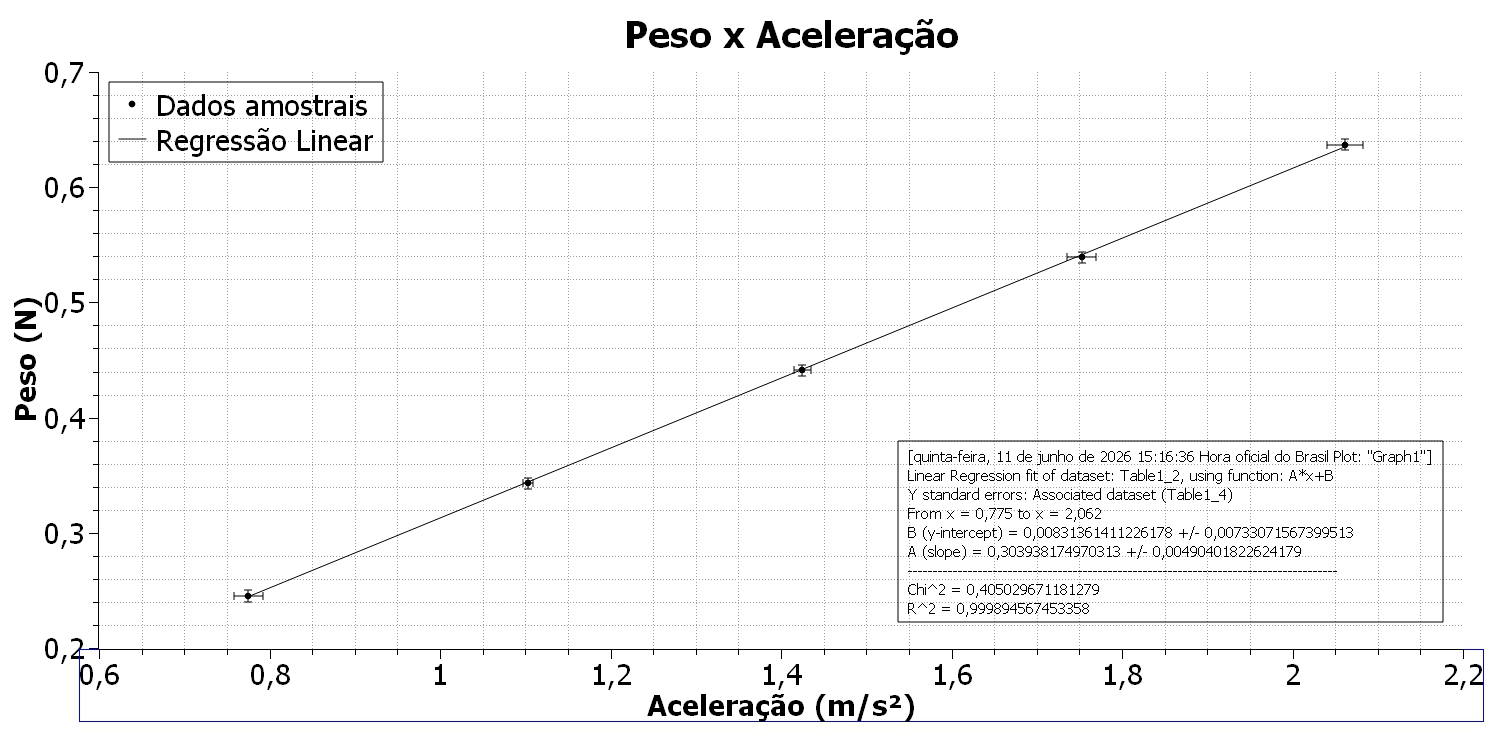
\includegraphics[width=9.5cm]{graf1.jpg}
	\caption{Galáxia Andrômeda no infravermelho}
	\label{fig1}
	\end{figure}
	\begin{figure}[!h]
	\centering
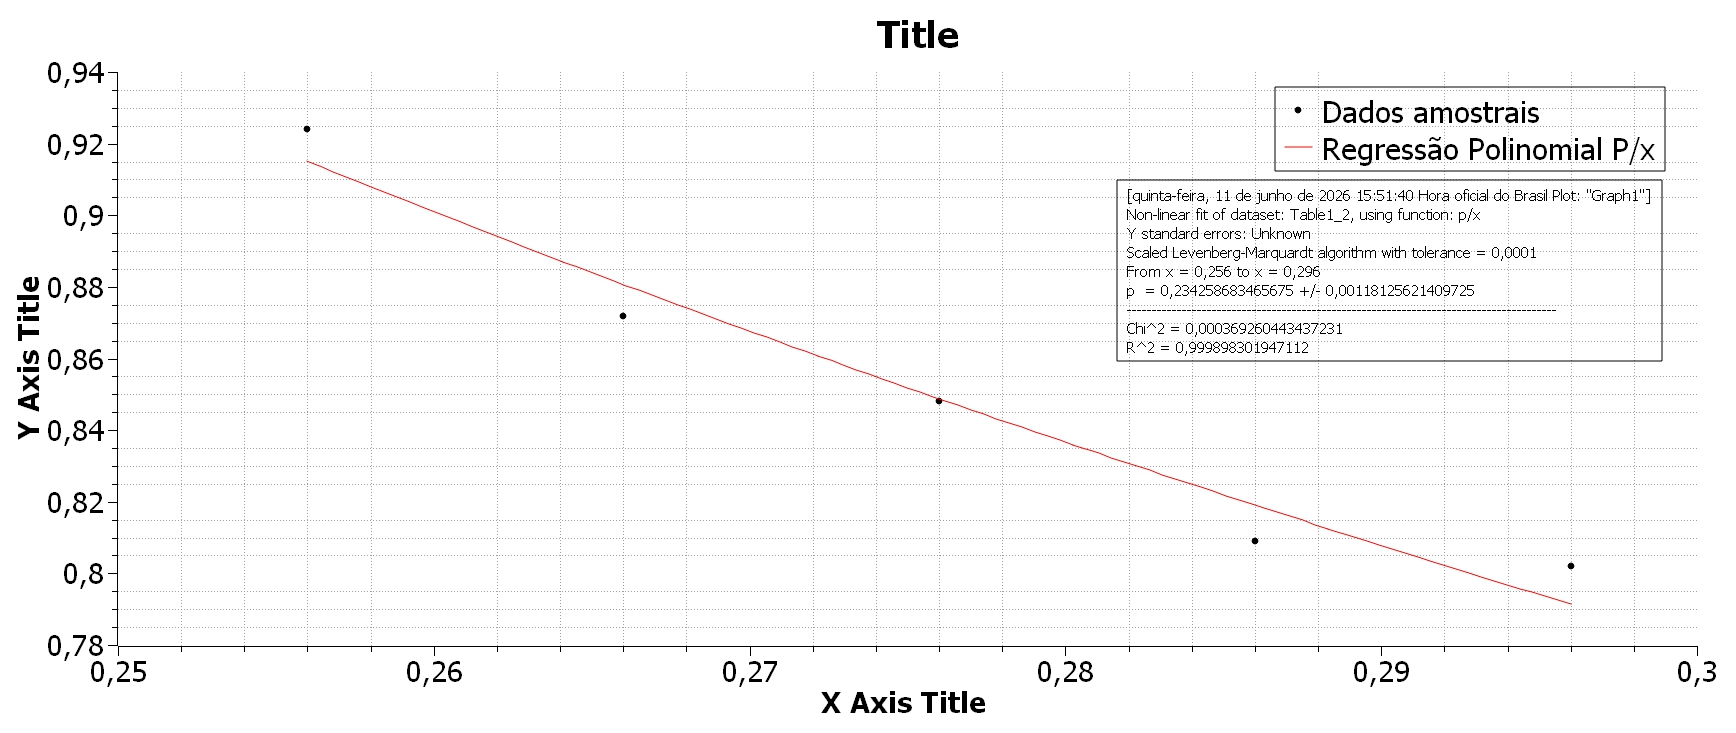
\includegraphics[width=9.5cm]{graf2.jpg}
	\caption{Diagrama do cronômetro, sensores, eletroímã e chave liga/desliga}
	\label{fig2}
	\end{figure}

\section{Conclusão}
Faça um resumo dos resultados finais obtidos, tomando os objetivos iniciais como referência.

%\section{Referências Bibliográficas}
\begin{thebibliography}{}
%\bibliography{basename of .bib file}
%Aqui são exemplos de como devem ficar as referências. Escrevam apenas as referências que foram utilizadas no experimento.

\bibitem{Wytler_1} Wytler C. Santos, {\it Roteiro do Experimento 1}, disponibilizado no portal UnB Aprender3.

\bibitem{Wytler_2} Wytler C. Santos, {\it Medidas, algarismos e erros}, texto disponibilizado no portal UnB Aprender3.

\bibitem {Young} H.D. Young \& R.A. Freedman, {\it Física I, Sears \& Zemansky}, Pearson, Addison Wesley, $12^a$ Ed., (2009).

\bibitem {Stefanelli_1} Eduardo J. Stefanelli, {\it Paquímetro universal virtual - simulador com nônio em milímetro 0,05 mm}

https://www.stefanelli.eng.br/paquimetro-virtual-simulador-milimetro-05/

\bibitem {Stefanelli_2} Eduardo J. Stefanelli, {\it Micrômetro virtual - simulador em milímetro centesimal}

https://www.stefanelli.eng.br/micrometro-virtual-milimetro-centesimal-simulador/




\end{thebibliography}



%\newpage

% \includepdf[pages=1]{Geometrodynamics.pdf} %%%%% Use esse comando se desejar acrescentar uma pagina em pdf




\end{document}
